\section{Experimental details}
\label{app:exp-details}

\paragraph{Adversarial line and adversarial clusters}
The following figure illustrates the adversarial distributions used in~\Cref{fig:list_size} and further in this section.
\begin{figure}[htbp]
    \centering
    \centering
    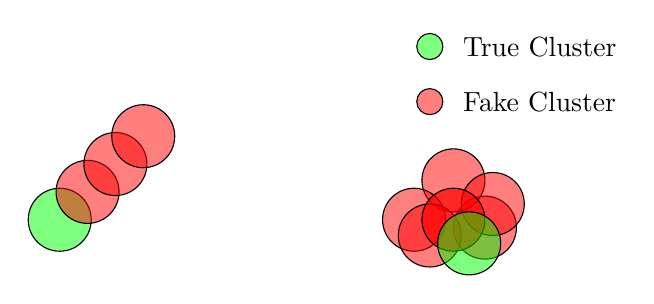
\begin{tikzpicture}
        % Adjust the opacity value as needed (between 0 and 1)
        \def\opacityValue{0.5}
    
        % Start a scope with rotation
        \begin{scope}[rotate=45]
            % Green circles (Good Gaussian Clusters)
            \node[draw, circle, fill=green, minimum size=0.8cm, fill opacity=\opacityValue] (green1) at (0,0) {};
            % \node[draw, circle, fill=green, minimum size=0.8cm, fill opacity=\opacityValue] (green2) at (2.5,0) {};
    
            % Red circles (Bad Gaussian Clusters) - Overlapping
            % Adjust the number of red circles and their positions as needed
            \foreach \x in {1,2,3}
                \node[draw, circle, fill=red, minimum size=0.8cm, fill opacity=\opacityValue] at (\x * 0.5,0) {};
        \end{scope}
    
        \def\horizontalShift{1.5}
    
        % Adjust the x-coordinate for each node using the parameter
        \node[draw, circle, fill=red, minimum size=0.8cm, fill opacity=\opacityValue] (green1) at ({3.9 + \horizontalShift}, -0.1) {};
        \node[draw, circle, fill=red, minimum size=0.8cm, fill opacity=\opacityValue] (green2) at ({3.5 + \horizontalShift}, 0.5) {};
        \node[draw, circle, fill=red, minimum size=0.8cm, fill opacity=\opacityValue] (green3) at ({3.0 + \horizontalShift}, 0) {};
        \node[draw, circle, fill=red, minimum size=0.8cm, fill opacity=\opacityValue] (green4) at ({4.0 + \horizontalShift}, 0.2) {};
        
        \node[draw, circle, fill=red, minimum size=0.8cm, fill opacity=\opacityValue] (green6) at ({3.2 + \horizontalShift}, -0.2) {};
        \node[draw, circle, fill=red, minimum size=0.8cm, fill opacity=0.7] (green7) at ({3.5 + \horizontalShift}, 0) {};
        \node[draw, circle, fill=green, minimum size=0.8cm, fill opacity=\opacityValue] (green5) at ({3.7 + \horizontalShift}, -0.3) {};
    
        % \draw[decoration={brace, amplitude=5mm, mirror}, decorate, rotate=45, line width=2pt]
        % (0.5,-0.5) -- (2.5,-0.5);
    
        % Add labels or content inside the curly braces if needed
        % \node at (2.1,0.2) {\Large\(\Delta\)};
    
        % Legend
        \node[draw, circle, fill=green, minimum size=0.3cm, fill opacity=\opacityValue] (legend1) at (4.7,2.2) {};
        \node[draw, circle, fill=red, minimum size=0.3cm, fill opacity=\opacityValue] (legend2) at (4.7,1.5) {};
        \node[right] at (5,2.2) {True Cluster};
        \node[right] at (5,1.5) {Fake Cluster};
\end{tikzpicture}
    
    \caption{Two variants of adversarial distribution: adversarial line (left) and adversarial clusters (right).}
    \label{fig:process_1}

\end{figure}


\paragraph{Data Distribution}
We consider a mixture of \(k = 7\) well-separated (\(\norm{\mu_i - \mu_j} \geq 40\)) \(d = 100\) dimensional inlier clusters whose subgroup sizes range from $0.3$ to $0.02$. The experiments are conducted once using a Gaussian distribution and once using a heavy-tailed t-distribution with five degrees of freedom for both inlier and adversarial clusters. In ~\Cref{fig:heavy_tailed_results} the latter suggests that our algorithm works comparatively well even for mixture distributions which do not fulfill our assumptions. We set \(\wmin = 0.02\) and \(\epsilon=0.12\) so that it is larger than the smallest clusters but smaller than the largest ones and set the total number of data points to \(10000\). The Gaussian noise model simply computes the empirical mean and covariance matrix of the clean data and samples \(1200\) noisy samples from a Gaussian distribution with this mean and covariance. The adversarial cluster model and the adversarial model are as depicted in~\Cref{fig:process_1}.

\begin{figure}[t]
    \centering
    \begin{minipage}[t]{0.8\linewidth}
        
\includegraphics[width=0.99\linewidth]{chapters/robust/figures/new_legend.pdf}
        \end{minipage}
    \begin{minipage}[t]{\linewidth}
        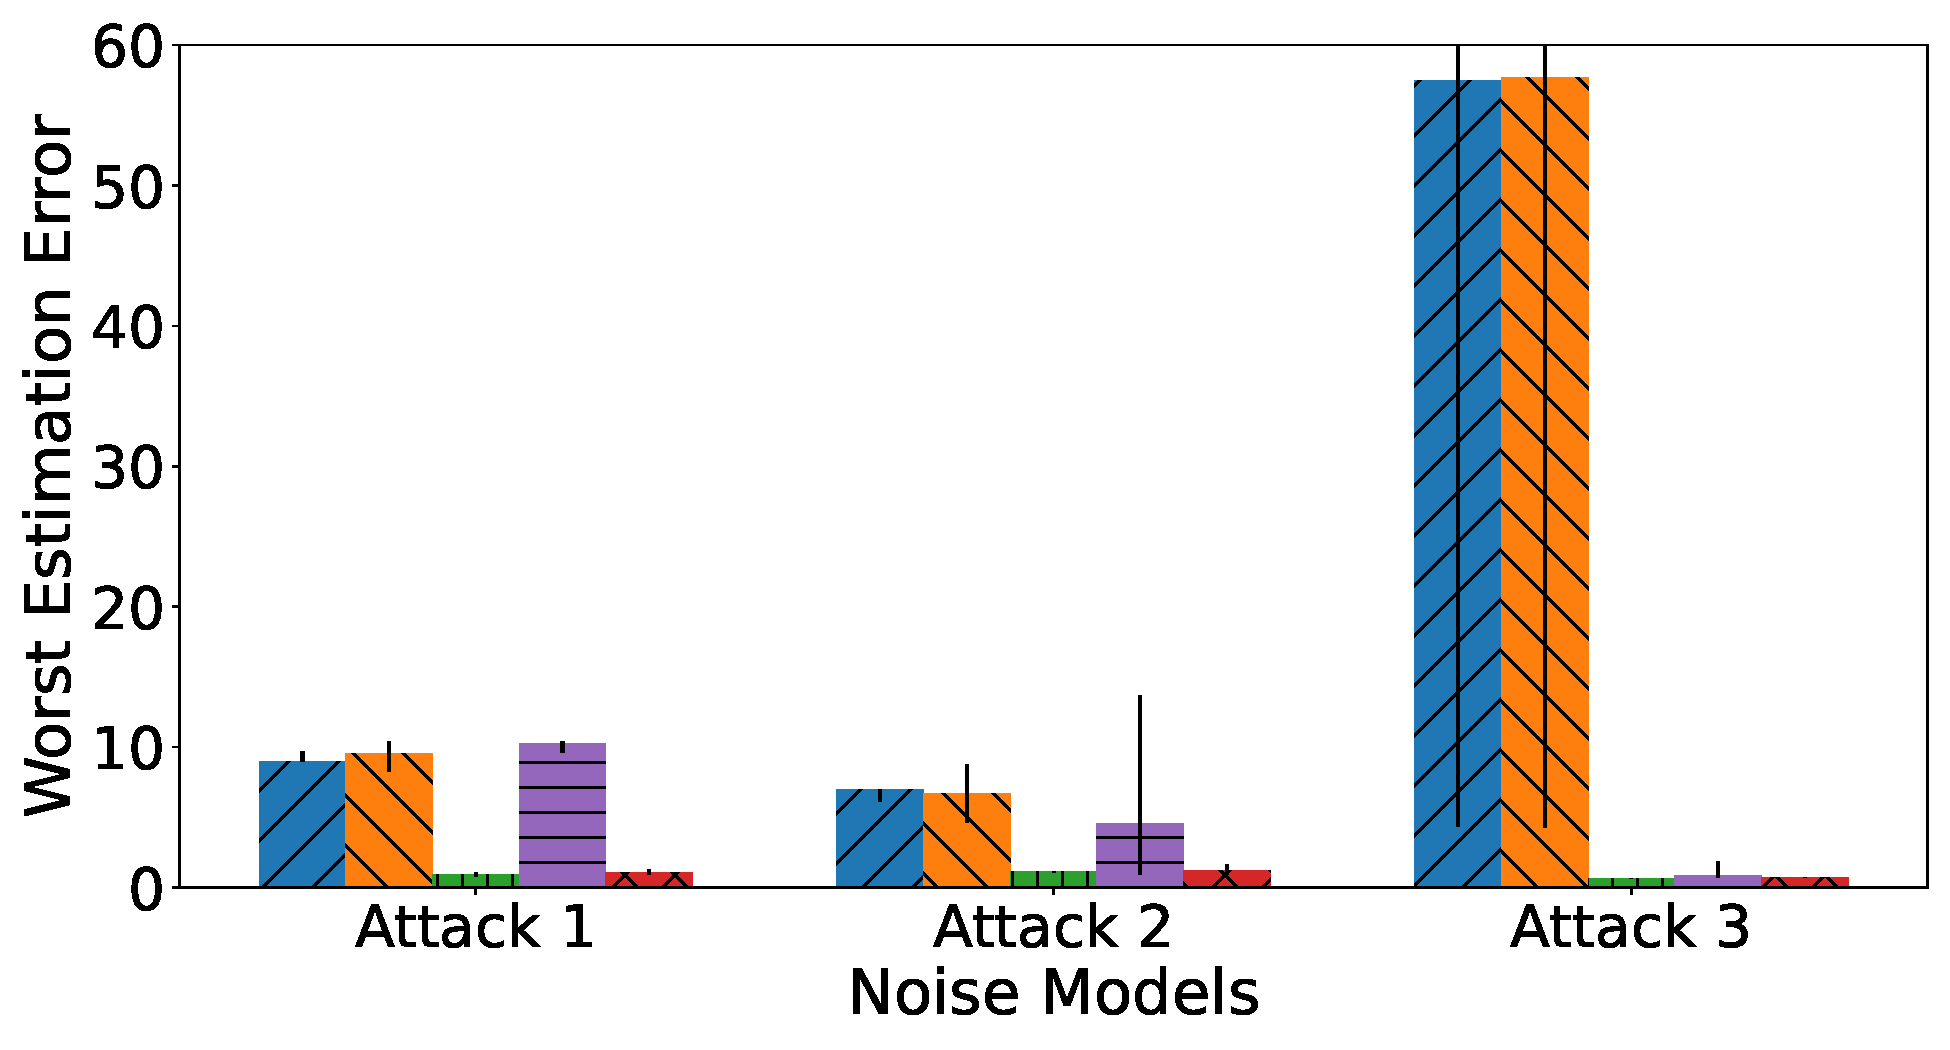
\includegraphics[width=0.49\linewidth]{chapters/robust/figures/gauss_inliers_3_attacks_error.pdf}
        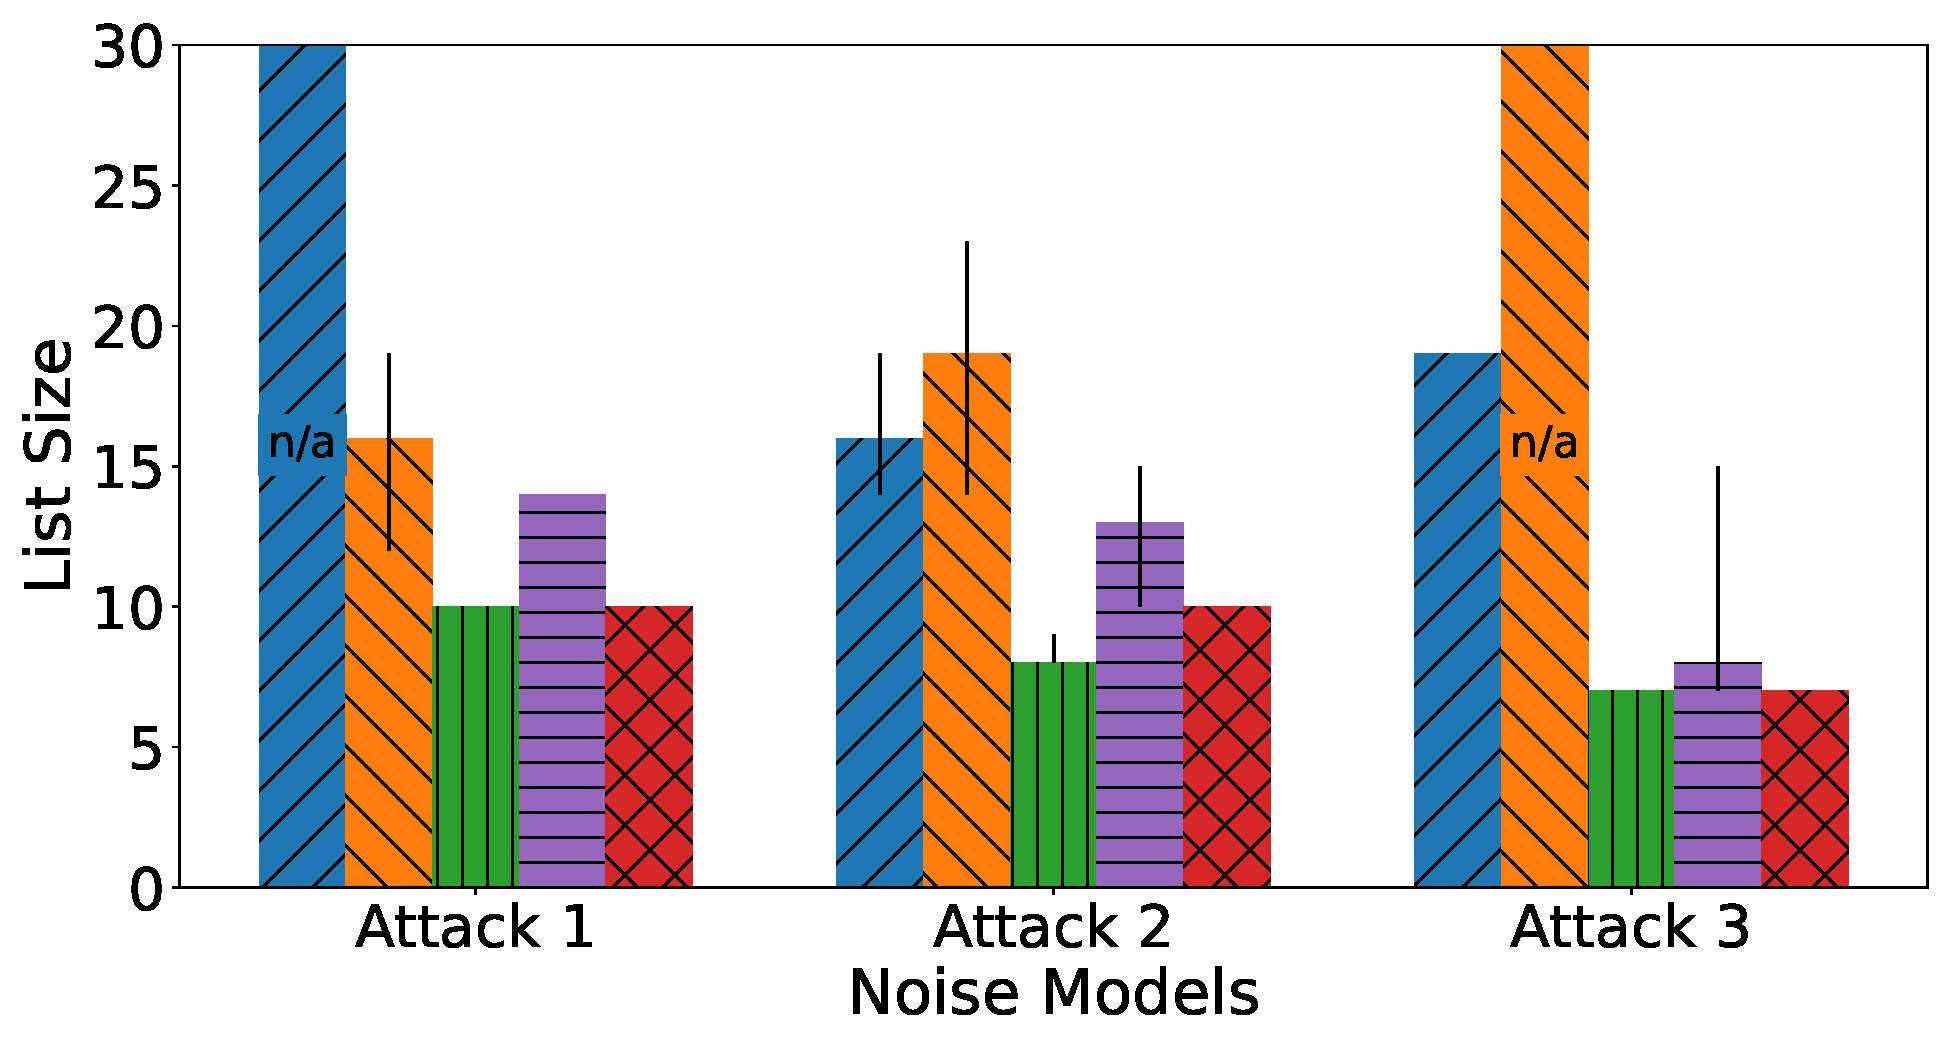
\includegraphics[width=0.49\linewidth]{chapters/robust/figures/gauss_inliers_3_attacks_size.pdf}
    \end{minipage}
    \caption{Comparison of five algorithms with three adversarial noise models. On the left we show worst estimation error of algorithms with constrained list size and on the right the smallest list size with constrained error guarantee.
    We plot the median of the metrics with the error bars showing \(25\)th and \(75\)th percentile. We observe that our method consistently outperforms prior works in terms of list size and worst estimation error, with the exception of DBSCAN, which performs at a similiar level.}
    \label{fig:err}
\end{figure}

\paragraph{Attack distributions}
We consider three distinct adversarial models (see~\Cref{fig:process_1} for reference).
\begin{enumerate}
    \item \emph{Adversarial clusters}: After sampling the inlier cluster means, we choose the cluster with the smallest weight. Let \(\mu_s\) denote its mean. Then, we sample a random direction \(v_c\) with \(\norm{v_c} = 10\). After that, we sample three directions \(v_1, v_2\) and \(v_3\) with \(\norm{v_i} = 10\). Then we put three additional (outlier) clusters with means at \(\mu_s + v_c + v_i\). This roughly corresponds to the right picture in~\Cref{fig:process_1}. The samples for each adversarial cluster are drawn from a distribution that matches the covariance of the inlier clusters, with the sample size being twice as large as of the affected inlier cluster.
    \item \emph{Adversarial line}: After sampling the inlier cluster means, we again choose the cluster with the smallest weight.
    Let \(\mu_s\) denote its mean. Then, we sample a random direction \(v_c\) with \(\norm{v_c} = 10\). 
    We put three additional (outlier) clusters with means at \(\mu_s + v_c, \mu_s + 2 v_c\) and \(\mu_s + 3v_c\), which form a line as shown in~\Cref{fig:process_1}. The samples are drawn similarly to the adversarial clusters, with the difference that the covariance is scaled by a factor of \(5\) in the direction of the line.
    \item \emph{Gaussian adversary}: Here we simply introduce noise matching the empirical mean and covariance of all inlier data (i.e., as if all inlier clusters are generated from the same Gaussian distribution).
\end{enumerate}
Note that in the first and second attack, the adversary creates clusters that do not respect the separation assumption of the true inlier clusters: either adversarial clusters are placed around the smallest inlier cluster (\textrm{Adversarial Cluster}), or the adversarial clusters form a line, pointing out in some fixed direction (\textrm{Adversarial Line}).

\paragraph{Implementation details}
We implement the list-decodable mean estimation base learner in our InnerStage algorithm (Algorithm \ref{alg:first_stage_high_level}) based on \cite{diakonikolas2022clustering}. It leverages an iterative multi-filtering strategy and one-dimensional projections. In particular, we use the simplified gaussian version of the algorithm. It is designed for distributions sampled from a Gaussian but also shows promising results for the experiments involving a heavy-tailed t-distribution as depicted in~\Cref{fig:heavy_tailed_results}. The robust mean estimator used to improve the mean hypotheses for large clusters is omitted in our implementation.

\begin{figure}[t]
    \centering
    \begin{minipage}[t]{0.8\linewidth}
        
\includegraphics[width=0.99\linewidth]{chapters/robust/figures/new_legend.pdf}
        \end{minipage}
    \begin{minipage}[t]{\linewidth}
        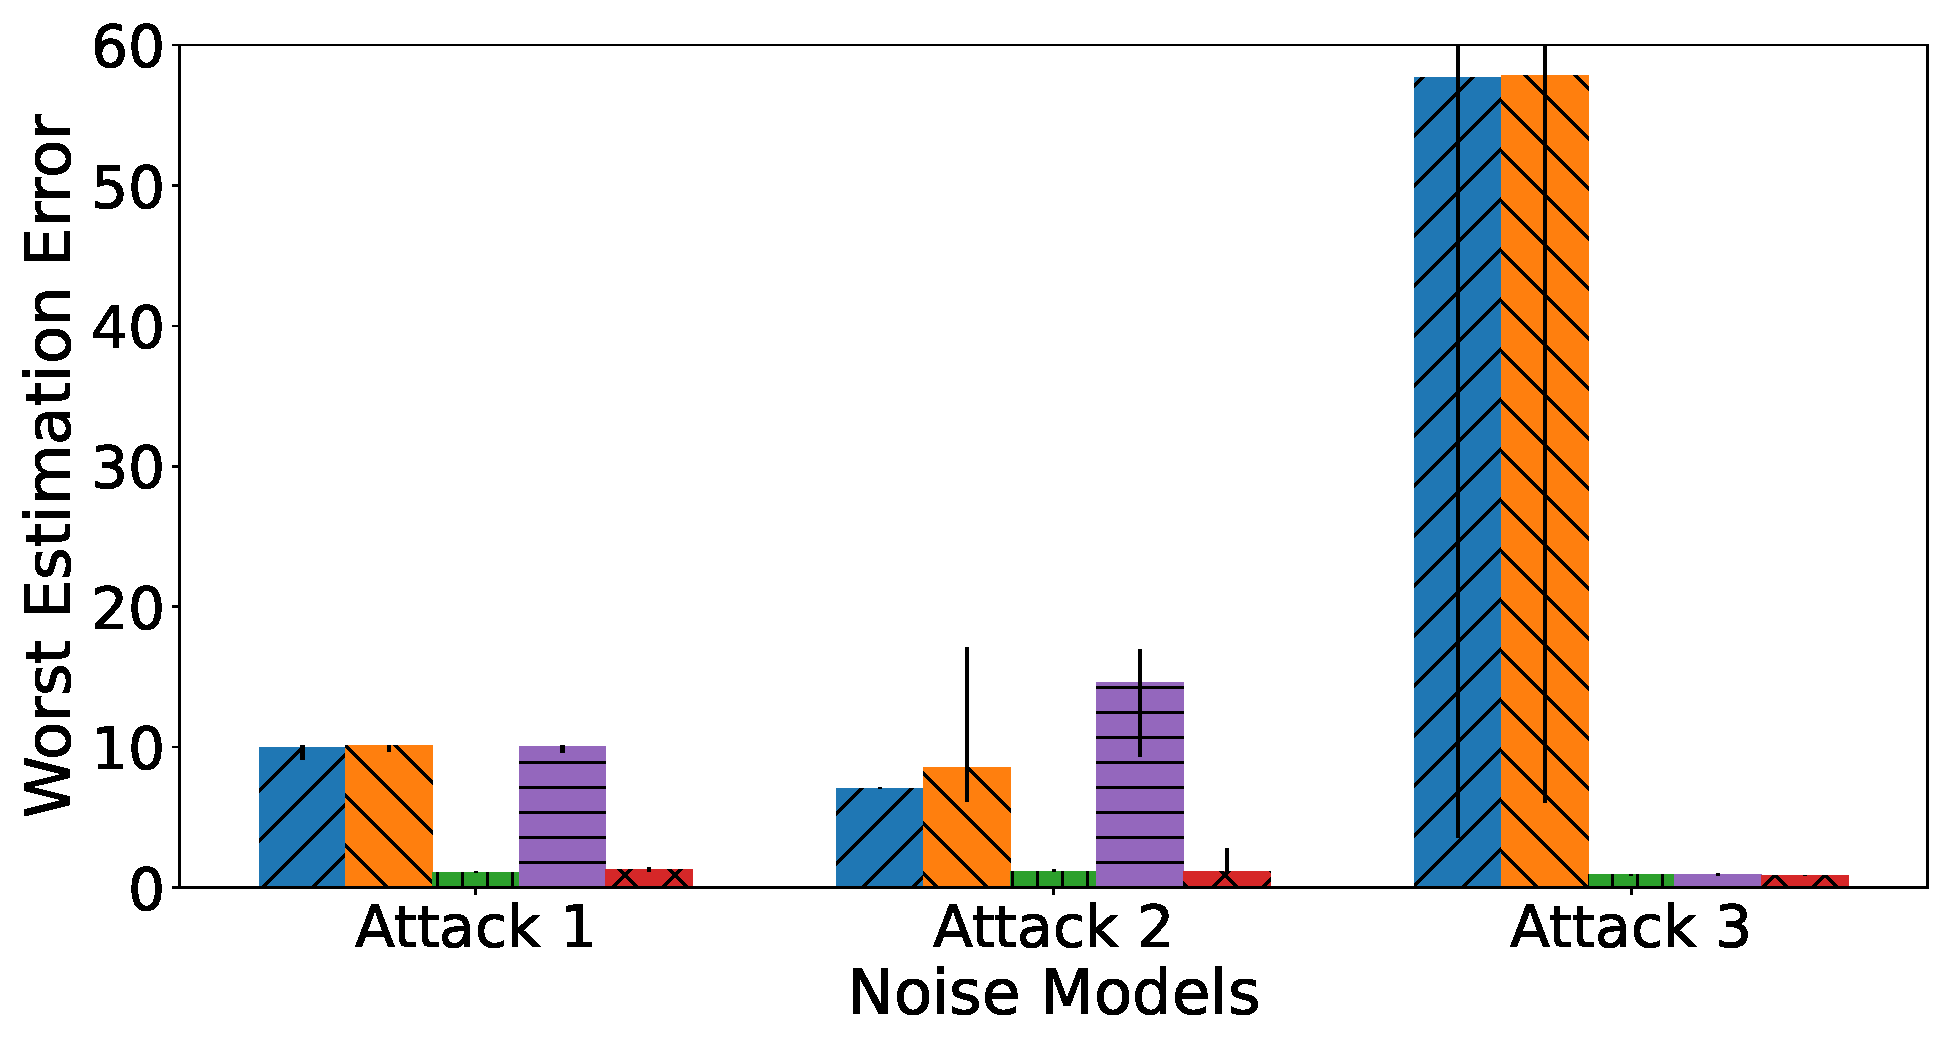
\includegraphics[width=0.49\linewidth]{chapters/robust/figures/tdist_inliers_3_attacks_error.pdf}
        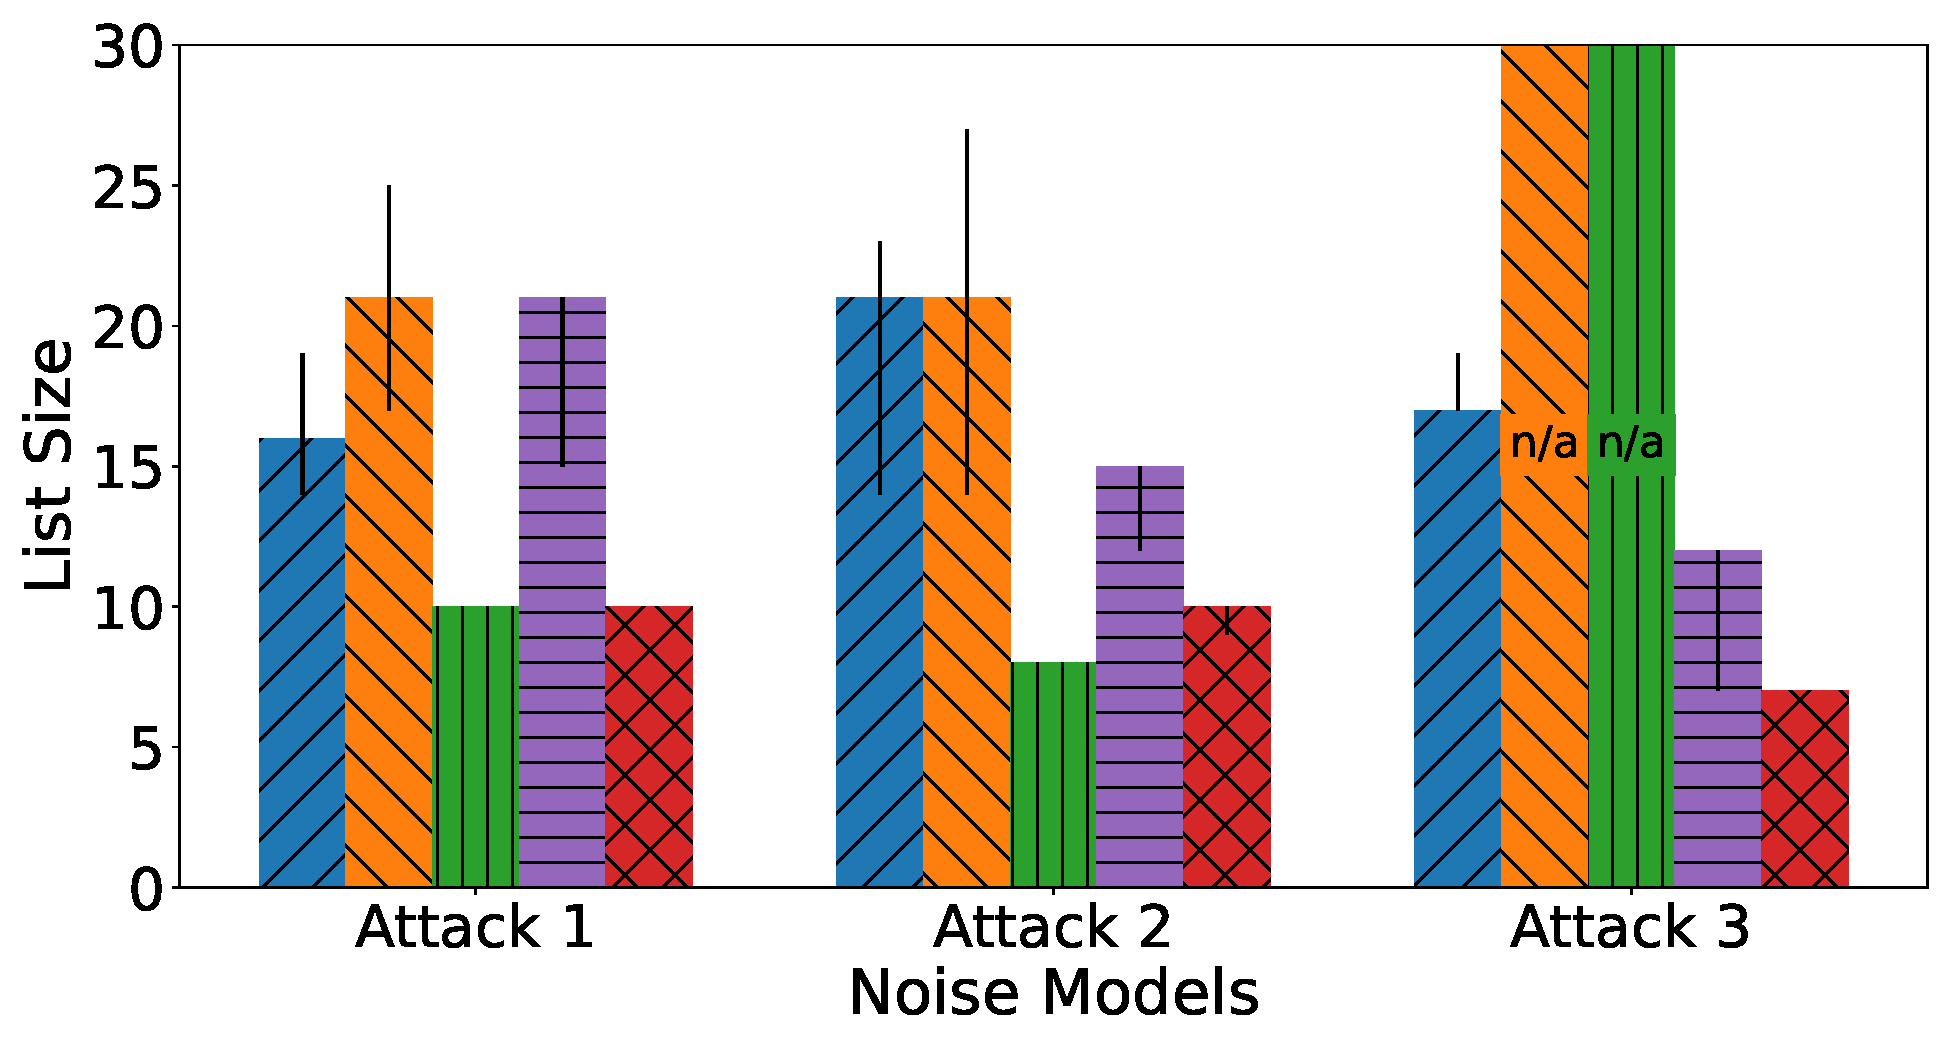
\includegraphics[width=0.49\linewidth]{chapters/robust/figures/tdist_inliers_3_attacks_size.pdf}
    \end{minipage}
    \caption{Worst estimation error and list size comparison for the case where inlier distributions are heavy-tailed. We can observe numerical stability of our approach.}
    \label{fig:heavy_tailed_results}
\end{figure}

\paragraph{Hyper-parameter search and experiment execution}
The hyper-parameters of our algorithm are tuned beforehand based on the experimental setup. For the comparative algorithms, hyper-parameter searches are conducted within each experiment after initial tuning. For our algorithm, key parameters include the pruning radius \(\gamma\) used in the OuterStage routine (Algorithm \ref{alg:second_stage_pruning}) and \(\beta\) used in the InnerStage (Algorithm \ref{alg:constructing_output}). In addition, parameters for the LD-ME base learner, such as the cluster concentration threshold, also require careful selection, resulting in a total of 7 parameters. The tuning for these was performed using a grid search comparing about \(250\) different configurations. Similarly, we independently tune the vanilla LD-ME algorithm, which we run with \(\wmin\) as weight parameter. For DBSCAN, we optimize the list size and error metrics by searching over a range of \(100\) values for \(\epsilon\), which controls the maximum distance between samples considered in the same neighbourhood. The minimum samples threshold, which validates the density based clusters, is pretuned beforehand and adjusted based on \(\wmin\). For \(k\)-means and its robust version, utilizing a median-of-means weighting scheme, we explore \(21\) values for \(k\), including the true number of clusters. 
Each parameter setting is executed \(100\) times to account for stochastic variations in the algorithmic procedures, such as \(k\)-means initialization. The list size and worst estimation error for each list of clusters obtained is visualized exemplarily for one iteration of the experiment in~\Cref{fig:scatter_plots}. The plot provides insight into how the different algorithms perform and vary with different list sizes.

\begin{figure}[t]
    \centering
    \begin{minipage}[t]{\linewidth}
        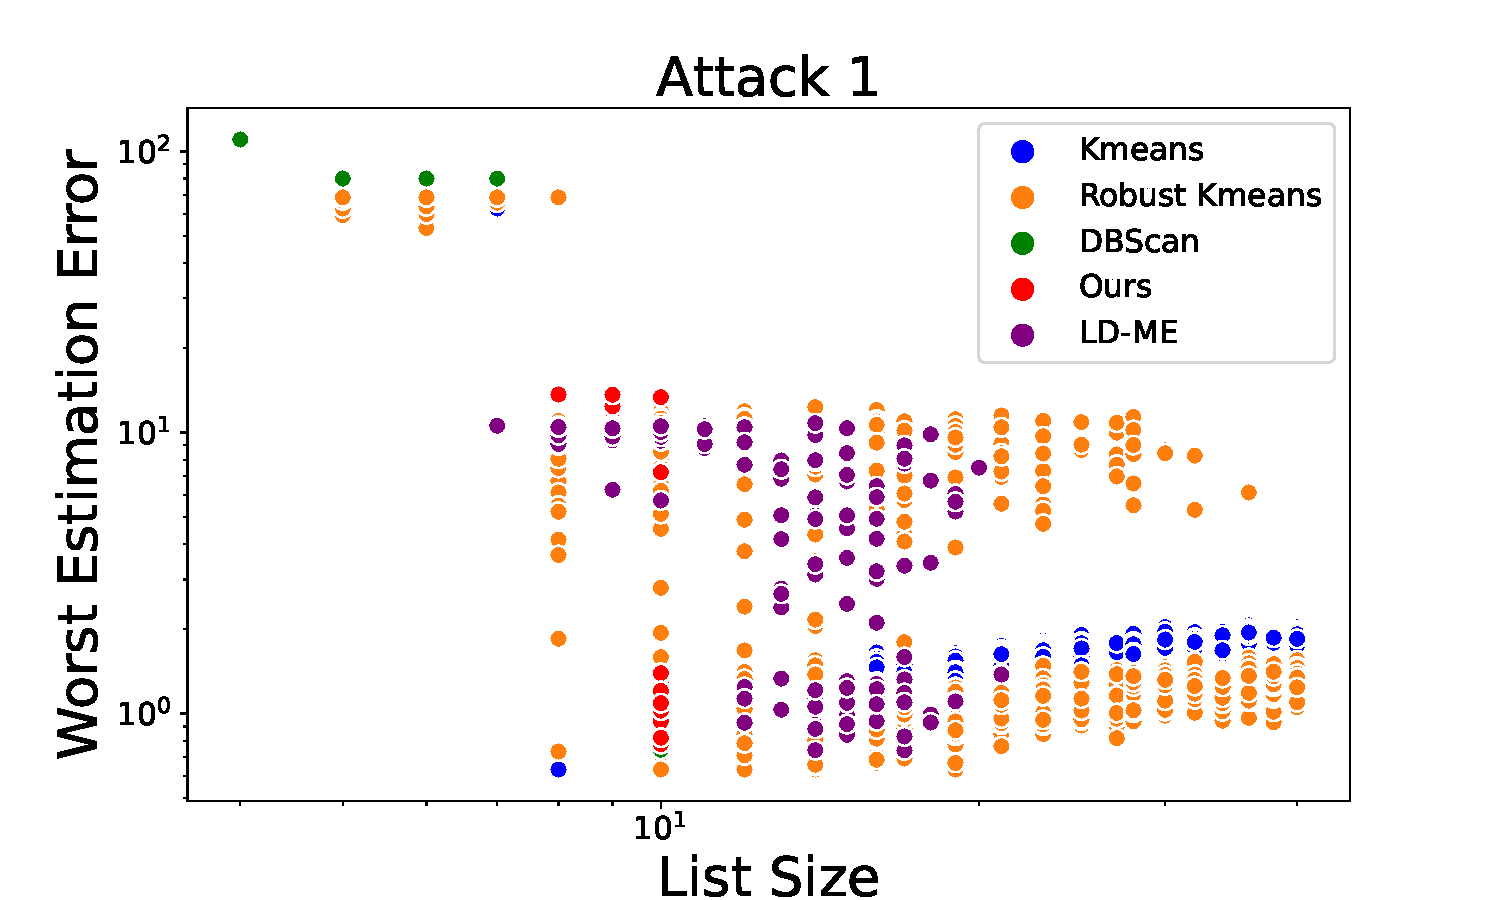
\includegraphics[width=0.4\linewidth]
        {chapters/robust/figures/gauss_inliers_adv_circle_scatter.pdf}
        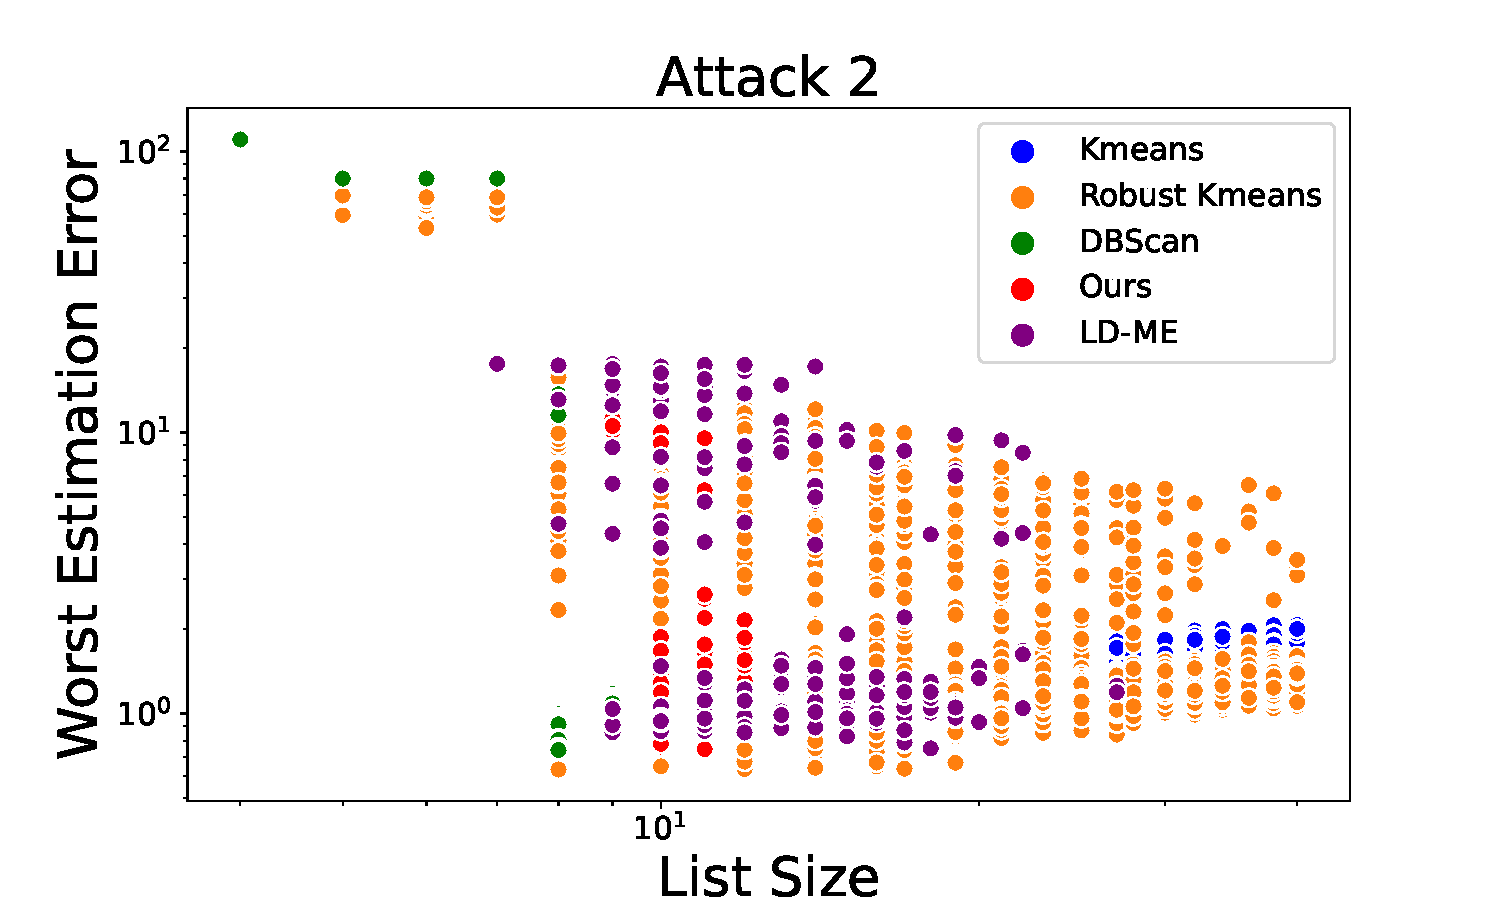
\includegraphics[width=0.4\linewidth]{chapters/robust/figures/gauss_inliers_adv_line_scatter.pdf}
    \end{minipage}
    \begin{minipage}[t]{\linewidth}
        \centering
        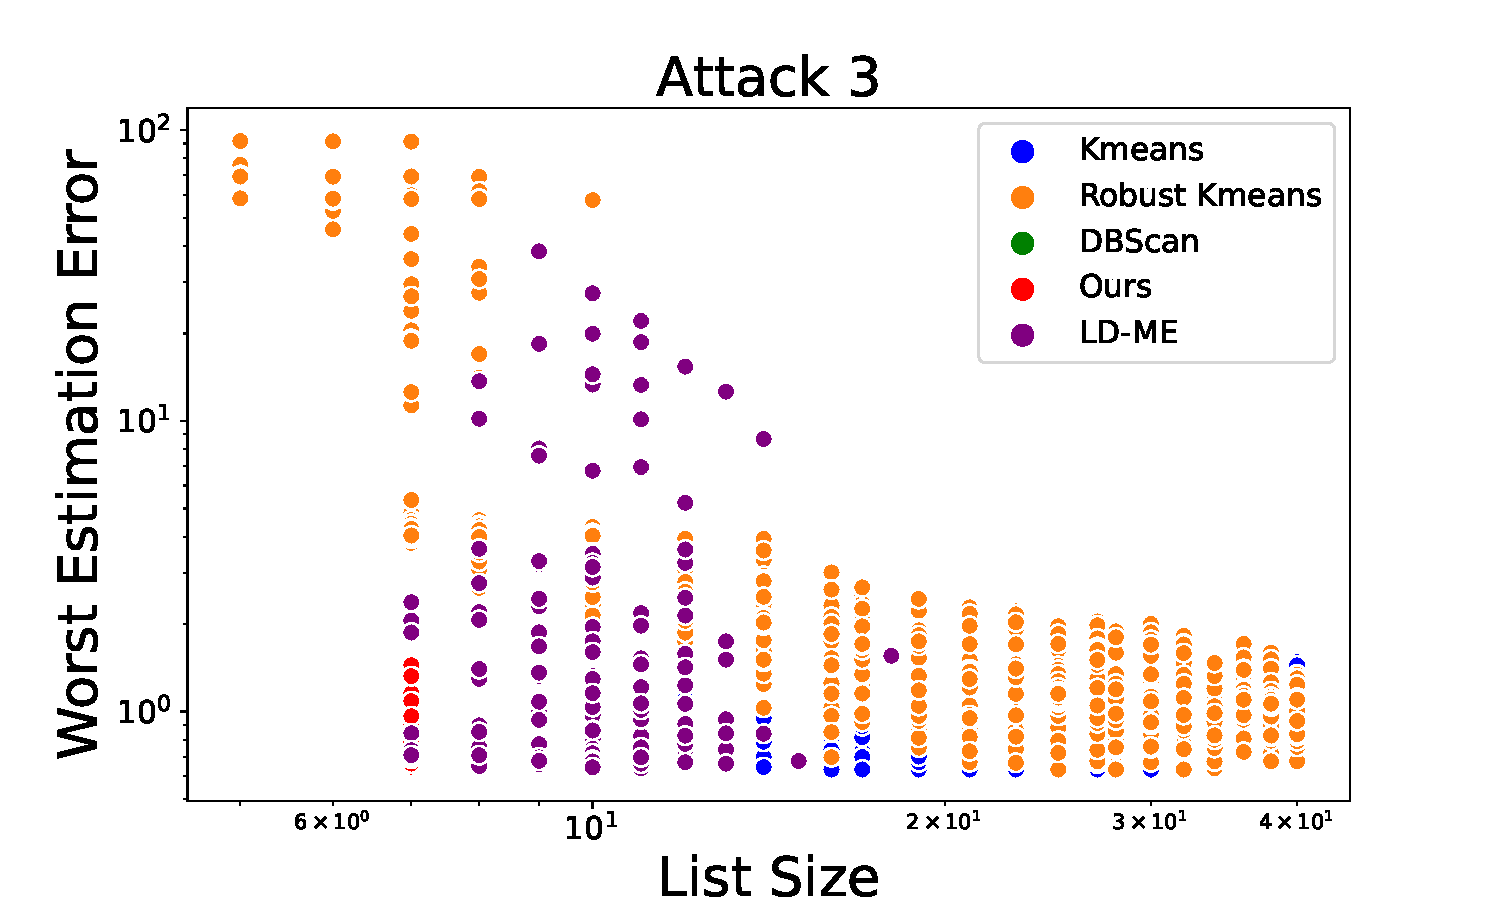
\includegraphics[width=0.4\linewidth]{chapters/robust/figures/gauss_inliers_gauss_noise_scatter.pdf}
    \end{minipage}
    \caption{Scatter plot of all results for one iteration of the experiment using three adversarial noise models.}
    \label{fig:scatter_plots}
\end{figure}

\paragraph{Evaluation details} 
Note that we have two sources of randomness: the data is random and also the algorithms themselves are random (except DBSCAN). For a clear comparison, we sample and fix one dataset for each attack model. 
we plot the performance of 
\(100\) runs of each algorithm for each parameter setting, % of the algorithms, 
each time recording the returned list size together with the worst estimation error \(\max_{i \in [k]} \min_{\muhat \in L} \norm{\mu_i - \muhat}\). Then we either (i) report the worst estimation error for all runs with constrained list size (we pick the list size most frequently returned by our algorithm, specifically \(7\) or \(10\) in our experiments) (see~\Cref{fig:err}, left), or (ii) report the smallest list size required to achieve the same or smaller worst estimation error (we pick the \(75\)th quantile of errors of our algorithm for a threshold) (see~\Cref{fig:err}, right).
Under size constraint (i), the bar plots correspond to the median over the runs, with error bars indicating  the \(25\)th and \(75\)th quantiles. Under error constraint (ii), the bar plots represent the minimum list size for which the median over the runs falls below the threshold, while the error bars show the minimum list size for which the \(25\)th and \(75\)th quantiles meet the constraint. Note that 'n/a' indicates that, within the scope of our parameter search, no list size achieves an error below the specified constraint.

In~\Cref{fig:heavy_tailed_results} we study the numerical stability of our approach. In particular, whether the performance degrades when inlier distribution does not satisfy required assumptions. We observe that if one uses our meta-algorithm with base learner designed for Gaussian inliers, we still obtain stable results even in the case of heavy-tailed inlier distribution.

\subsection{Variation of \(\wmin\)}
\label{sec:app-wlow}
To study the effect of varying \(\wmin\) input on the performance of our approach and LD-ME, we introduce a new noise model. As illustrated in ~\Cref{fig:wlow_variation_setup}, we consider a mixture of \(k = 3\) well-separated clusters: one small cluster with a weight of \(0.045\) and two large clusters, each with a weight of \(0.2\). We place two adversarial clusters (see paragraph on attack distributions for details): one near the small cluster and another near one of the large clusters. Furthermore, uniform noise is introduced, spanning the range of the data generated by the inlier and its nearby outlier cluster and accounting for \(10\%\) of the data in this region. Overall, \(\epsilon = 0.56\) and we draw \(22650\) samples from this mixture distribution.

For both algorithms we run 100 seeds for each \(\wmin\) ranging from 0.02 to 0.2, which corresponds to the weight of the largest inlier cluster. In ~\Cref{fig:wlow_variation}, we plot the median estimation error with error bars showing the \(25\)th and \(75\)th quantiles for the small cluster (top left) and the large cluster near the outlier cluster (top right). As expected from our theoretical results, we observe that our algorithm performs roughly constant in estimating the mean of the large cluster, regardless of the initial \(\wmin\). Meanwhile, the estimation error of LD-ME increases as \(\wmin\) decreases further below the true cluster weight. Furthermore, the plots show that our approach does consistently outperform LD-ME in terms of both worst estimation error and list size. ~\Cref{fig:wlow_variation_bar_plots} also compares the performance of the clustering algorithms in this experimental setup with results similar to the ones obtained in the previous experimental settings. 

\subsection{Computational resources}
Our implementation of the algorithm and experiments leverages multi-threading. It utilizes CPU resources of an internal cluster with \(128\) cores, which results in a execution time of about \(5\) minutes for a single run of the experiment for one noise model with \(10000\) samples. We remark that classic approaches like \(k\)-means and DBSCAN perform fast and the most time-consuming part is the execution of the LD-ME base learner. Given our experimental setup with three noise models, it takes about \(15\) minutes to reproduce all our results for one data distribution.

\begin{figure}[hb]
    \centering
    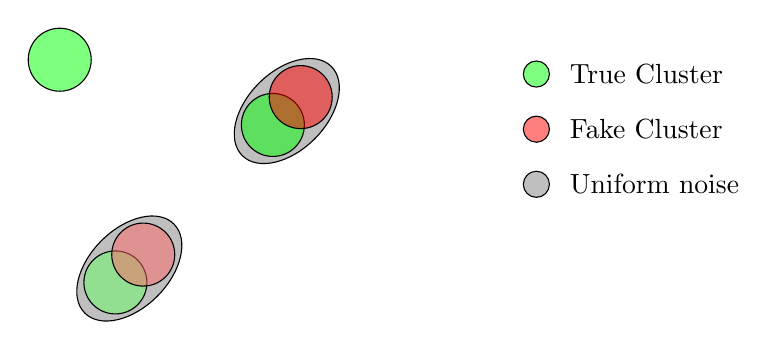
\begin{tikzpicture}
        % Adjust the opacity value as needed (between 0 and 1)
        \def\opacityValue{0.5}
    
        % Start a scope with rotation
        \begin{scope}[rotate=45]
            % uniform noise covering both circles
            \draw[fill=gray, fill opacity=\opacityValue] (0.75, 0) ellipse (0.8cm and 0.5cm);
            
            % Green circles (Good Gaussian Clusters)
            \node[draw, circle, fill=green, minimum size=0.8cm, fill opacity=\opacityValue] (green1) at (0.5,0) {};
    
            % Red circles (Bad Gaussian Clusters) - Overlapping
            \node[draw, circle, fill=red, minimum size=0.8cm, fill opacity=\opacityValue] at (1,0) {};

        \end{scope}

        \begin{scope}[shift={(-2, -2)}, rotate=45]
            % uniform noise covering both circles
            \draw[fill=gray, fill opacity=\opacityValue] (0.75, 0) ellipse (0.8cm and 0.5cm);
            
            % Green circles (Good Gaussian Clusters)
            \node[draw, circle, fill=green!60, minimum size=0.8cm, fill opacity=\opacityValue] (green1) at (0.5,0) {};

            \node[draw, circle, fill=green, minimum size=0.8cm, fill opacity=\opacityValue] (green1) at (2,2.5) {};
    
            % Red circles (Bad Gaussian Clusters) - Overlapping
            \node[draw, circle, fill=red!60, minimum size=0.8cm, fill opacity=\opacityValue] at (1,0) {};

        \end{scope}
    
        % Legend
        \node[draw, circle, fill=green, minimum size=0.3cm, fill opacity=\opacityValue] (legend1) at (3.7,1) {};
        \node[draw, circle, fill=red, minimum size=0.3cm, fill opacity=\opacityValue] (legend2) at (3.7,0.3) {};
        \node[draw, circle, fill=gray, minimum size=0.3cm, fill opacity=\opacityValue] (legend3) at (3.7, -0.4){};
        \node[right] at (4,1) {True Cluster};
        \node[right] at (4,0.3) {Fake Cluster};
        \node[right] at (4, -0.4) {Uniform noise};
        
\end{tikzpicture}
    
    \caption{Setup for \(\wmin\) variation experiment with clusters contaminated by an adversarial cluster and uniform noise. Lower color intensities indicate smaller cluster weights.}
    \label{fig:wlow_variation_setup}
\end{figure}

\begin{figure}[hb]
    \centering
    \begin{minipage}[t]{\linewidth}
        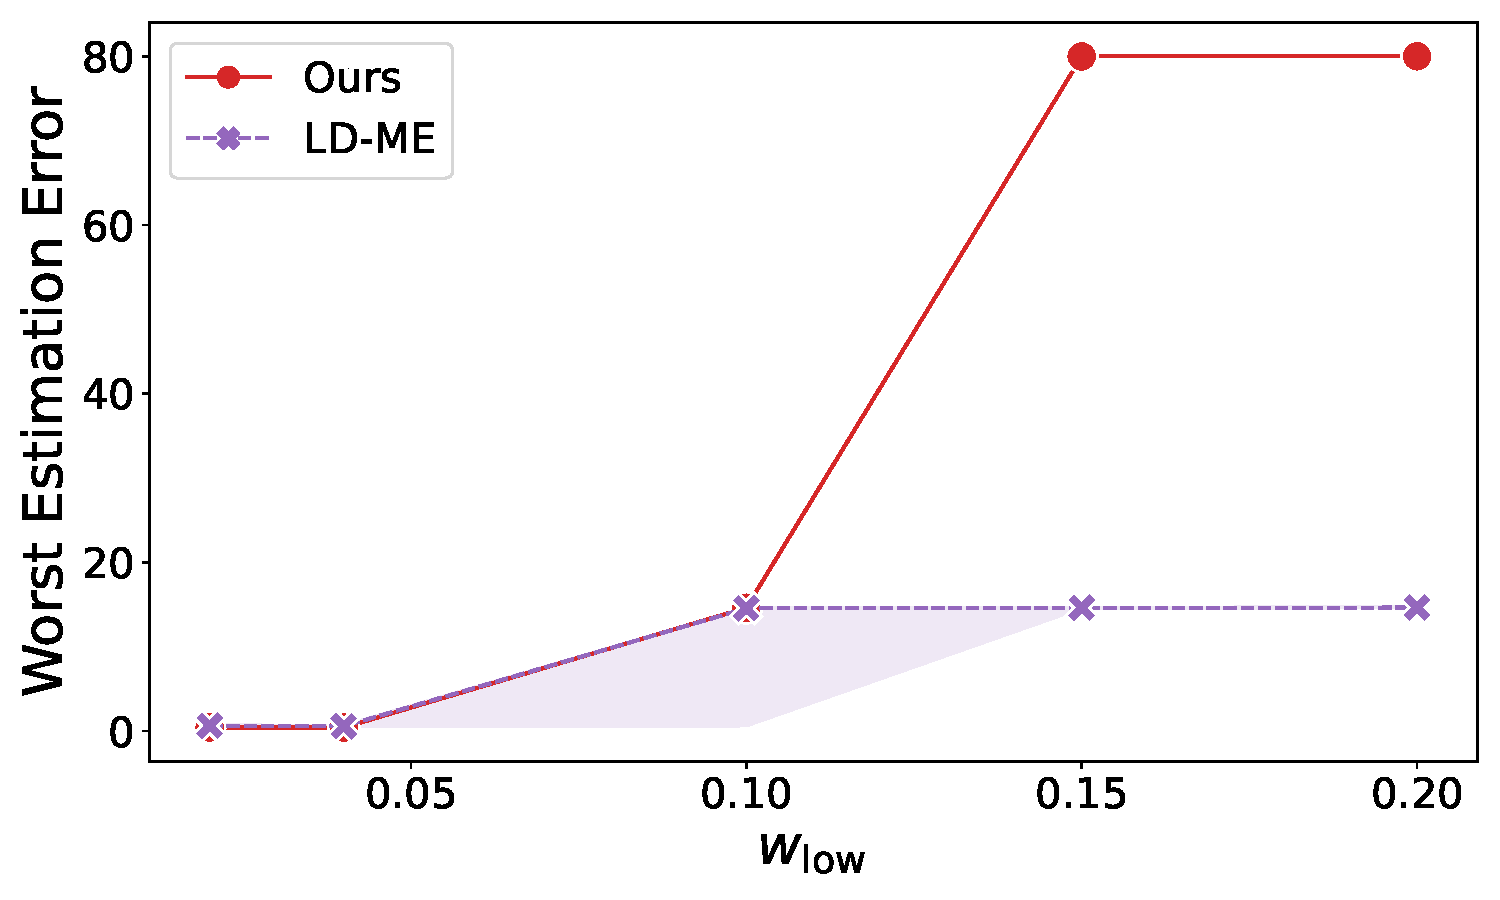
\includegraphics[width=0.4\linewidth]
        {chapters/robust/figures/wlow_variation_error_small.pdf}
        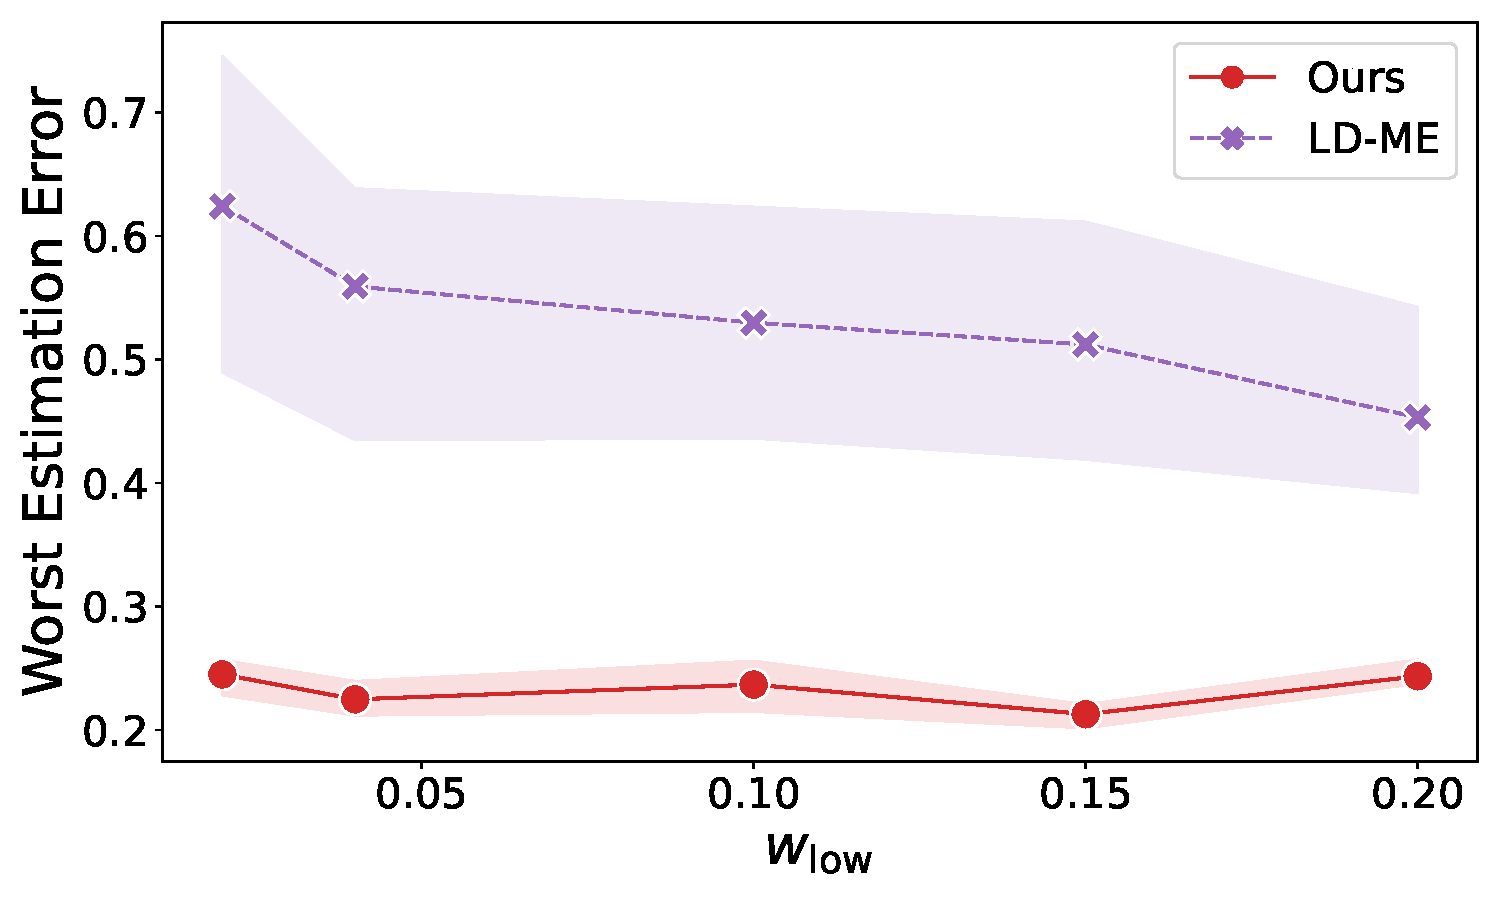
\includegraphics[width=0.4\linewidth]{chapters/robust/figures/wlow_variation_error_large.pdf}
    \end{minipage}
    \begin{minipage}[t]{\linewidth}
        \centering
        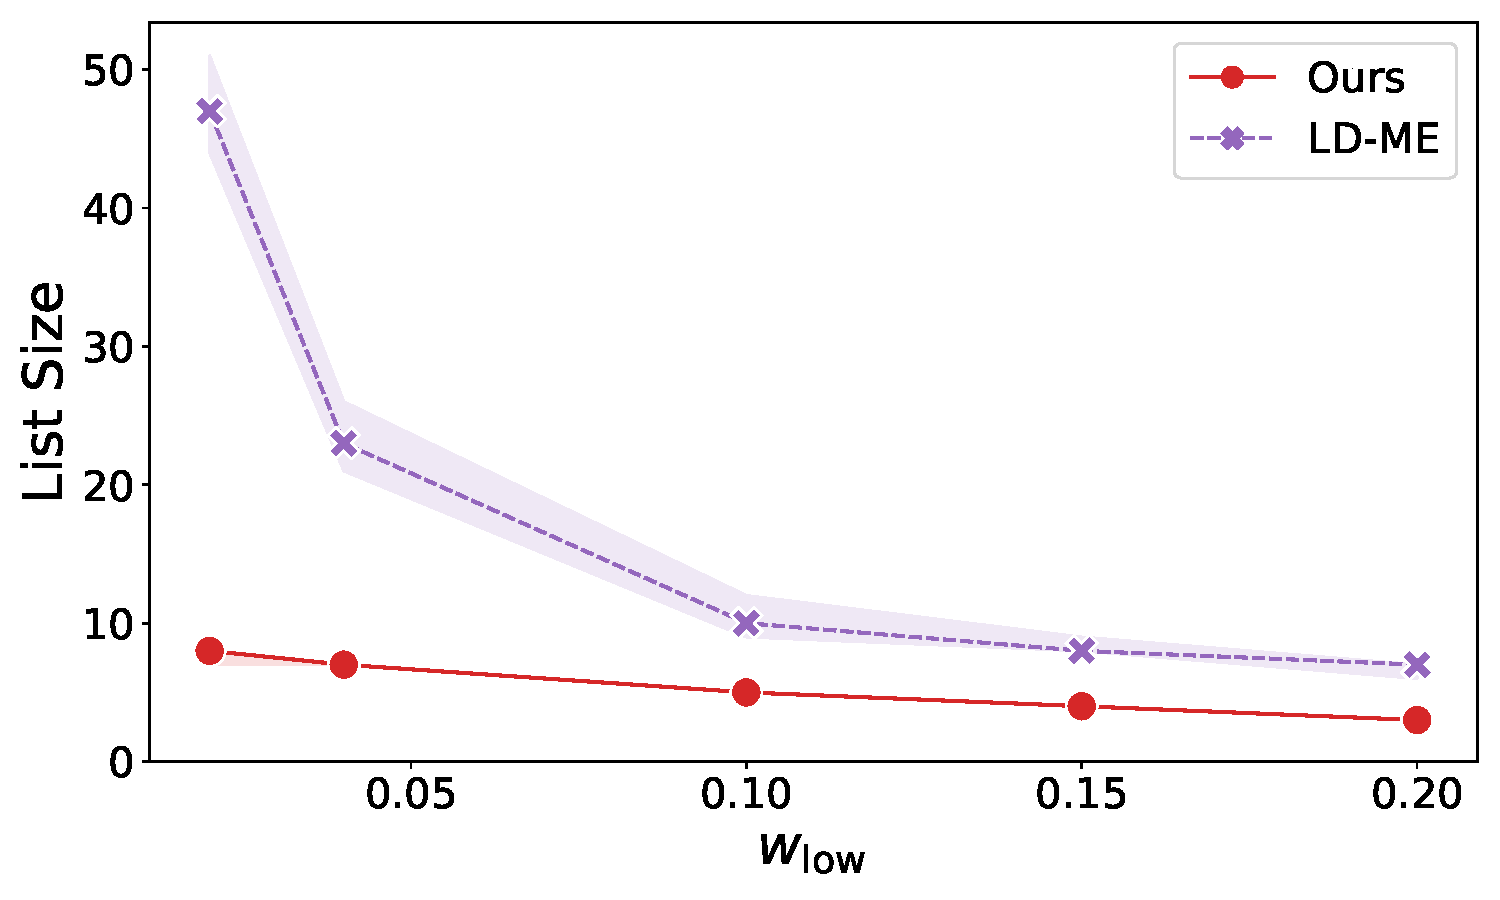
\includegraphics[width=0.4\linewidth]{chapters/robust/figures/wlow_variation_size.pdf}
    \end{minipage}
    \caption{Comparison of list size and estimation error for small and large inlier clusters for varying \(\wmin\) inputs. The experimental setup is illustrated in~\Cref{fig:wlow_variation_setup}. The plot on the top left shows the estimation error for the small cluster and the plot on the top right shows the error for the large cluster. We plot the median values with error bars indicating 25th and 75th quantiles. As \(\wmin\) decreases, our algorithm maintains a roughly constant estimation error for the large cluster, while the error for LD-ME increases.}
    \label{fig:wlow_variation}
\end{figure}

\begin{figure}[b]
    \centering
    \begin{minipage}[t]{\linewidth}
        \centering
        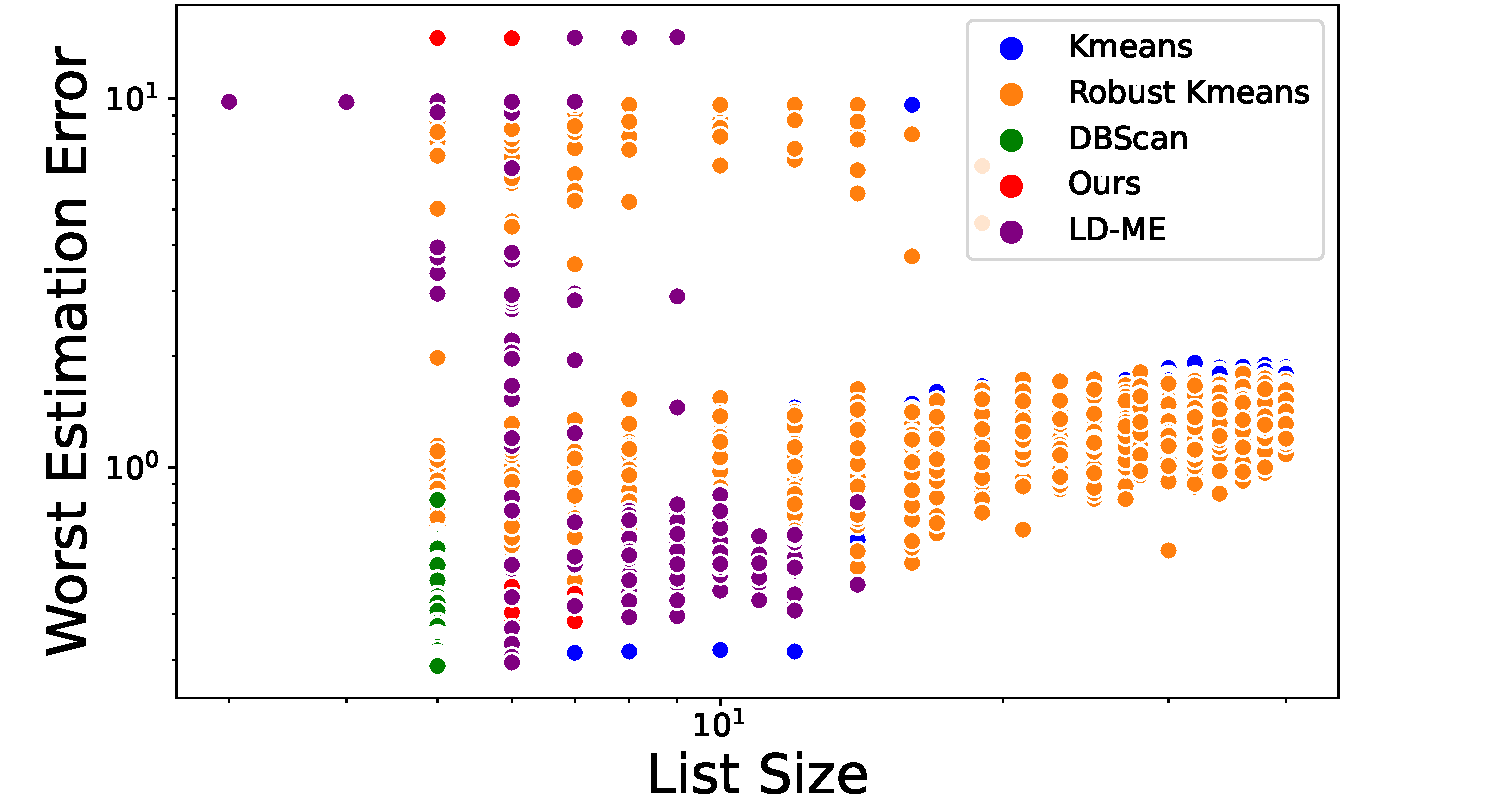
\includegraphics[width=0.4\linewidth]{chapters/robust/figures/wlow_variation_scatter_cropped.pdf}
        \vspace{3mm}
    \end{minipage}
    \begin{minipage}[t]{0.8\linewidth}
        
\includegraphics[width=0.99\linewidth]{chapters/robust/figures/new_legend.pdf}
        \end{minipage}
    \begin{minipage}[t]{\linewidth}
        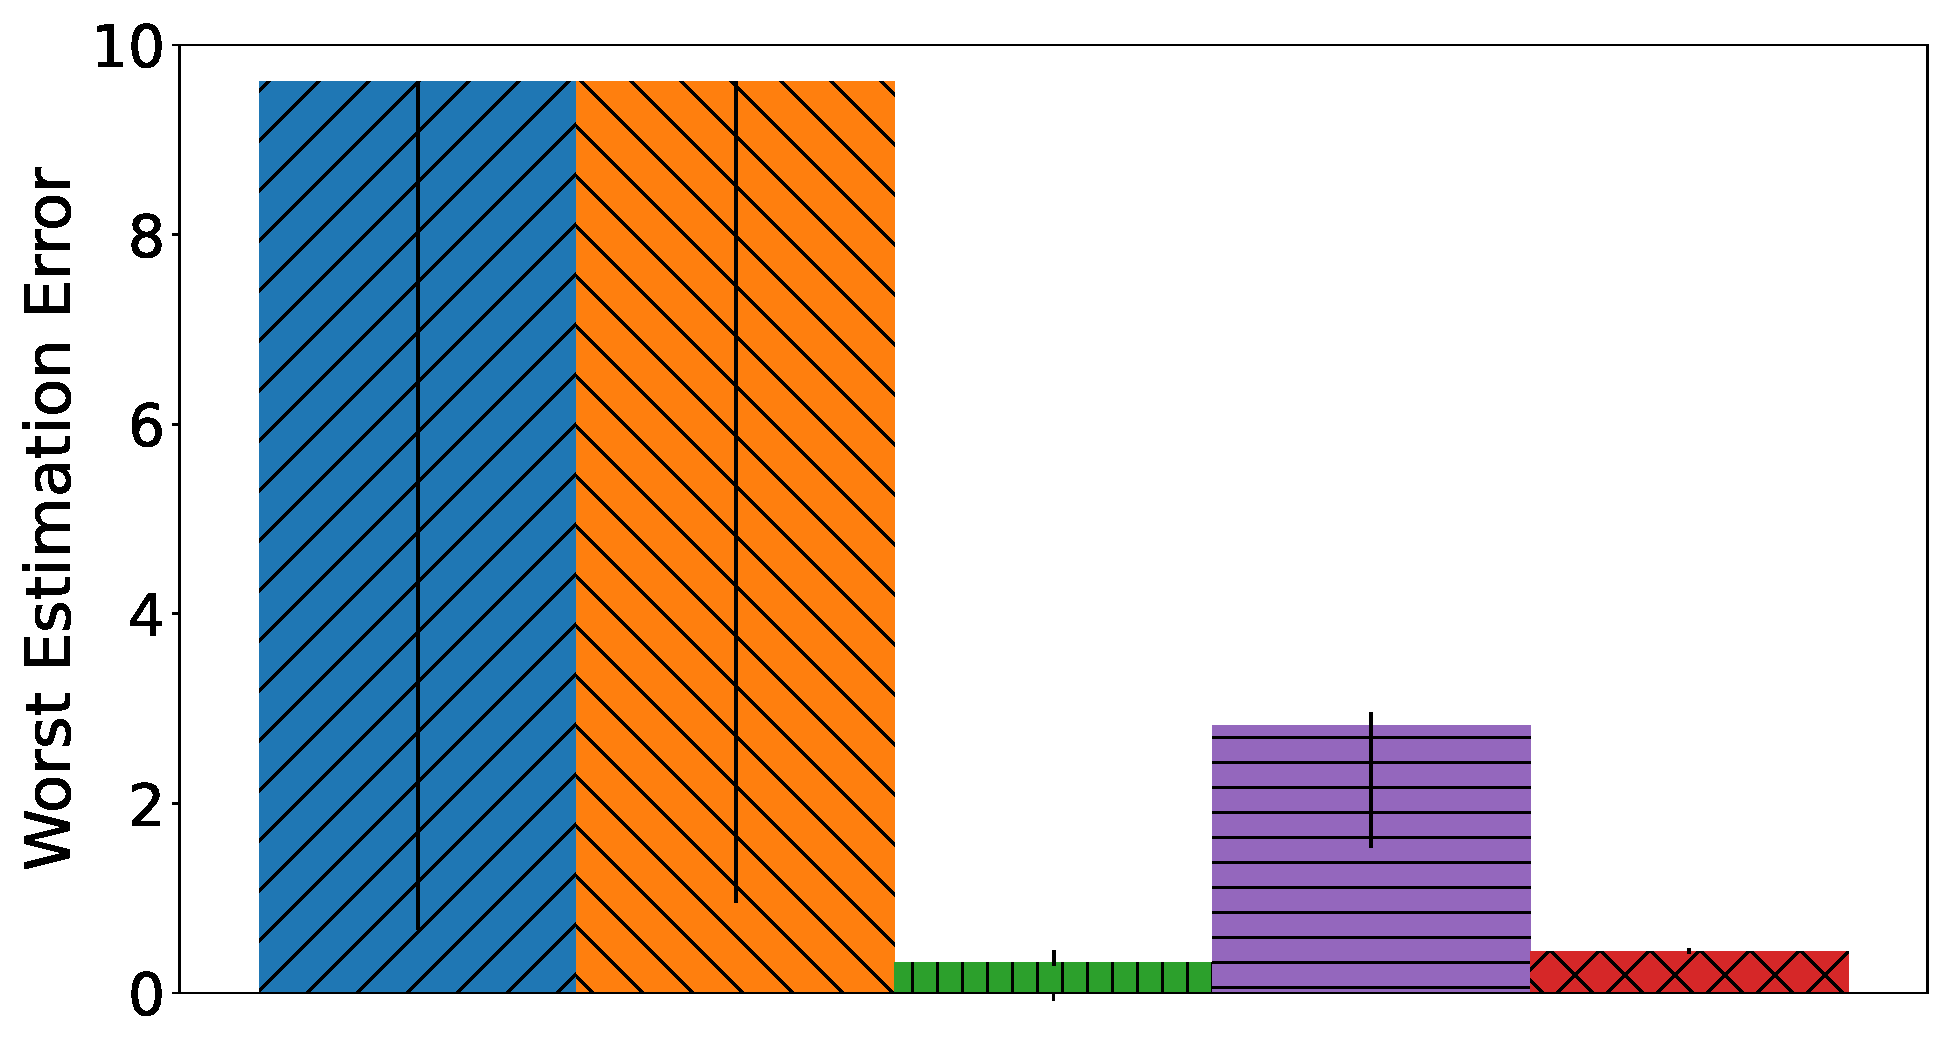
\includegraphics[width=0.4\linewidth]{chapters/robust/figures/wlow_variation_1_attack_error.pdf}
        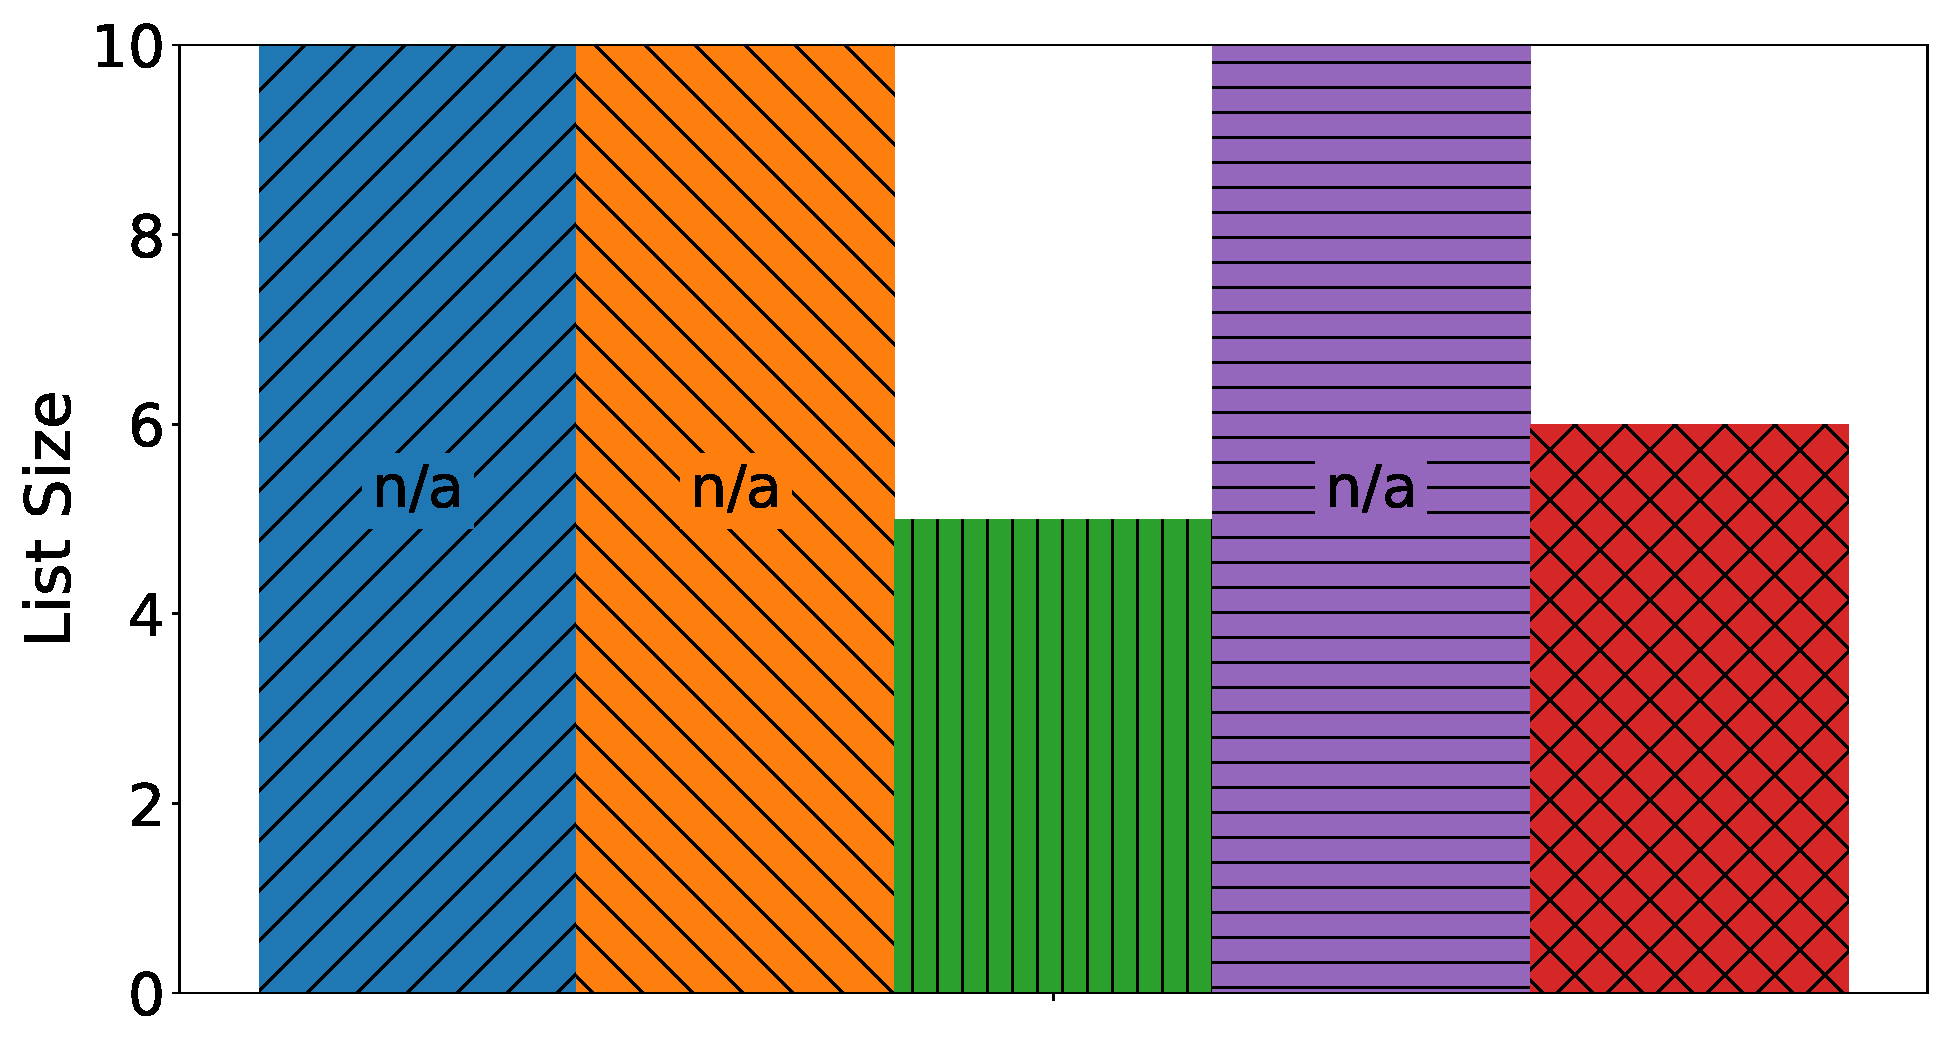
\includegraphics[width=0.4\linewidth]{chapters/robust/figures/wlow_variation_1_attack_size.pdf}
    \end{minipage}
    \caption{Worst estimation error and list size comparison for the setup used in the \(\wmin\) variation experiment.}
    \label{fig:wlow_variation_bar_plots}
\end{figure}

